\section{HTTP}
Despite the security provided by TLS, the websites themselves can still be vulnerable to attacks.
Especially if the wrong website is accessed, or the website is not properly secured.

\begin{Def}[HTML - HyperText Markup Language Elaboration]

    \label{def:html}
    \textbf{HTML} (HyperText Markup Language) is the standard markup language used for creating and structuring content on the web. HTML provides a system of elements (tags) that describe the structure and content of a webpage.
    
    \begin{itemize}
        \item HTML documents are made up of \textbf{elements}, which consist of:
        \begin{enumerate}
            \item Opening tags (e.g., \texttt{<p>} for a paragraph),
            \item Content (text, images, links, etc.), and
            \item Closing tags (e.g., \texttt{</p>}).
        \end{enumerate}
        \item The structure of an HTML document includes:
        \begin{itemize}
            \item \textbf{Head Section:} Metadata, title, and links to external resources.
            \item \textbf{Body Section:} Visible content such as headings, paragraphs, images, and links.
        \end{itemize}
    \end{itemize}
    
    \noindent HTML is the backbone of webpages and works alongside CSS for styling and JavaScript for interactivity.
    \end{Def}

    \noindent
    The task know is to understand the structure of an HTML document. Just like with any software, someone had to program it.
    Even the best of programers can make mistakes, these mistakes open up backdoors and vulnerabilities in the software. 
    Such vulnerabilities can be exploited by attackers to gain access to the system.

    \begin{theo}[Schneier's Law]

        \label{theo:schneier}
        \begin{quote}
            \emph{``Any person can invent a security system so clever that they can't imagine a way of breaking it.''}
        \end{quote}

        \vspace{.5em}
        \noindent
        Human ingenuity has its limits. If one vulnerability exists, there are bound to be more. \hfill
    \end{theo}

    \newpage
    
\begin{Example}[HTML Structure]
The following is an example of a basic HTML document:

\begin{verbatim}
<!DOCTYPE html>
<html lang="en">
<head>
    <meta charset="UTF-8">
    <meta name="viewport" content="width=device-width, initial-scale=1.0">
    <title>My First HTML Page</title>
</head>
<body>
    <h1>Hello, World!</h1>
    <p>This is my first paragraph.</p>
    <a href="https://www.example.com">Visit Example</a>
</body>
</html>
\end{verbatim}

\noindent
\textbf{Explanation:}
\begin{itemize}
    \item \texttt{<!DOCTYPE html>} declares the document type.
    \item The \texttt{<html>} element is the root of the document.
    \item The \texttt{<head>} section contains metadata and the page title.
    \item The \texttt{<body>} section includes visible content like headings, paragraphs, and links.
\end{itemize}
\end{Example}

\begin{theo}[Content Loading in HTTP and HTTPS]

    \label{theo:http_https_loading}
    When a user requests a webpage over \textbf{HTTP} or \textbf{HTTPS}, the browser does not load the page as a single entity. Instead, the following process occurs:
    \begin{enumerate}
        \item The initial \textbf{skeleton of the page} (HTML) is fetched from the primary server.
        \item The browser identifies and requests any \textbf{linked resources}, such as:
        \begin{itemize}
            \item Images, videos, and scripts (e.g., \texttt{<img>}, \texttt{<script>}),
            \item Stylesheets (e.g., \texttt{<link rel="stylesheet">}),
            \item Fonts or third-party resources (e.g., analytics, ads, or widgets).
        \end{itemize}
        \item These subsequent resources may originate from \textbf{multiple servers or domains}, even if the user initially visited a single site.
    \end{enumerate}
    \end{theo}

    \newpage 

\begin{theo}[Multiple Requests Implications]

    Despite visiting one site, the user's browser may establish connections to \textbf{several servers}, often unknowingly. This introduces potential security and privacy concerns, such as:
    \begin{itemize}
        \item Content loaded over insecure connections (HTTP) may compromise the integrity of the page.
        \item Third-party services can track user behavior across different sites.
    \end{itemize}
    
\end{theo}
    
\begin{Example}[Multiple Requests in Practice]
Suppose a user visits \texttt{https://example.com}. The server provides the main HTML document. The browser then identifies and fetches linked resources, such as:
\begin{verbatim}
GET https://example.com/index.html       (main page)
GET https://cdn.example.com/style.css    (stylesheet)
GET http://images.example.com/logo.png  (image)
GET https://ads.thirdparty.com/ad.js     (third-party script)
\end{verbatim}
Here, the user's browser interacts with \texttt{example.com}, \texttt{cdn.example.com}, \texttt{images.example.com}, and \texttt{thirdparty.com}.

\noindent
As a result, the user's session involves multiple servers, illustrating the distributed nature of webpage loading.
Here the \textbf{images} being accessed are over \textbf{HTTP}, which can compromise the integrity of the page.
\end{Example}

\begin{theo}[HTTPS Enforcement in Modern Browsers]

    \label{theo:https_enforcement}
    Modern websites and browsers enforce the use of \textbf{HTTPS} connections to ensure secure communication between the client and server. This includes:
    \begin{itemize}
        \item \textbf{Client-Side Enforcement:}  
        Most browsers block mixed content (HTTP resources on HTTPS pages) and warn users against accessing HTTP-only sites.
        \item \textbf{Server-Side Enforcement:}  
        Websites implement HTTP Strict Transport Security (HSTS) to automatically upgrade all connections to HTTPS and prevent insecure fallback.
    \end{itemize}
    
    \noindent By requiring HTTPS, both client and server reduce risks of eavesdropping, tampering, and impersonation, ensuring confidentiality, integrity, and authenticity of the data exchanged.
\end{theo}
    

\newpage 
\begin{Def}[Tracking Pixels]

    \label{def:tracking_pixels}
    A \textbf{tracking pixel} (also known as a web beacon, pixel tag, or 1x1 pixel) is a small, transparent image or code snippet (typically \texttt{1x1} pixels in size) embedded in emails, webpages, or advertisements. It is used to track user behavior and collect data about interactions.
    
    \begin{itemize}
        \item \textbf{How It Works:}
        \begin{enumerate}
            \item The tracking pixel is hosted on a server.
            \item When a user loads the webpage or opens an email, the browser requests the pixel from the server.
            \item This request contains metadata such as:
            \begin{itemize}
                \item IP address of the user,
                \item Device and browser information,
                \item Time of access, and
                \item Referrer URL.
            \end{itemize}
        \end{enumerate}
    
        \item \textbf{Purpose:} Tracking pixels are primarily used for:
        \begin{itemize}
            \item \textbf{Analytics:} Measuring email open rates, ad impressions, and user engagement.
            \item \textbf{Behavioral Tracking:} Monitoring user activity on websites or across advertising campaigns.
            \item \textbf{Personalization:} Collecting data to tailor ads or content to specific users.
        \end{itemize}
    
        \item \textbf{Privacy Implications:}  
        Tracking pixels can operate without explicit user consent, raising concerns about:
        \begin{itemize}
            \item User privacy and data collection without awareness,
            \item Cross-site tracking by third-party advertisers.
        \end{itemize}
    \end{itemize}
\end{Def}

\begin{Example}[Tracking Pixel in HTML]
    A tracking pixel is typically implemented as an invisible image hosted on a remote server:
    
    \begin{verbatim}
    <img src="https://tracking.example.com/pixel" width="1" height="1"
    alt="" style="display:none;">
    \end{verbatim}
    
    \noindent
    When this HTML is loaded, the browser requests the pixel from the server. The server records metadata such as the user's IP address, browser type, and referrer.
\end{Example}

\newpage

\noindent
Everything is code, if one wishes to search something on the internet.
Some server has to take the users response, interpret it, and send back the results.
This interaction with the internal code opens the door for attack vectors.

\begin{theo}[Injection Attacks]

    \label{theo:injection_attacks}
    An \textbf{Injection Attack} occurs when an adversary provides malicious input to a system, exploiting the way user data is processed and interpreted by internal code. This attack vector leverages the fact that systems often interact with external inputs, such as databases, command interpreters, or web applications.
    
    \begin{itemize}
        \item \textbf{Mechanism:} The attacker injects crafted data that is processed as executable code or commands, causing unintended behavior such as:
        \begin{itemize}
            \item Executing unauthorized commands,
            \item Accessing sensitive data,
            \item Manipulating system operations.
        \end{itemize}
   
        \item \textbf{Mitigation:} Strong input validation, parameterized queries, and escaping special characters are key defenses against injection attacks.
    \end{itemize}
\end{theo}

\begin{theo}[Cross-Site Scripting (XSS)]
    \label{theo:xss}
    \textbf{Cross-Site Scripting (XSS)} is a type of injection attack where an adversary injects malicious scripts into trusted websites, causing the browser to execute them on behalf of the victim. 
    
    \begin{itemize}
        \item \textbf{Mechanism:} 
        XSS exploits vulnerabilities in web applications that fail to properly sanitize user inputs. The attacker injects malicious code into webpages or inputs, which is then executed in the context of the victim's browser.
    
        \item \textbf{Impact:} 
        XSS attacks can lead to user session hijacking, defacement of webpages, or unauthorized data access.
    
        \item \textbf{Types of XSS:}
        \begin{itemize}
            \item \textbf{Stored XSS:} Malicious scripts are permanently stored on the server and executed whenever the resource is accessed.
            \item \textbf{Reflected XSS:} The script is reflected off a web server, typically via a URL parameter or input field.
            \item \textbf{DOM-Based XSS:} The script is executed directly in the browser, manipulating the Document Object Model (DOM) without server-side interaction.
        \end{itemize}
    \end{itemize}
    
\end{theo}
    

    
\newpage
\begin{Example}[SQL Injection on a Login Page]
    \textbf{Scenario:}
    A login page allows users to enter a username and password. The server processes these inputs using a vulnerable SQL query. An attacker probes the system to identify weaknesses and then injects malicious SQL to bypass authentication.
    
    \textbf{Initial Probe:} The attacker enters \texttt{' OR 1=1--} in the username field to test if the input is sanitized.
    \begin{verbatim}
    Input:
        Username: ' OR 1=1--
        Password: (leave blank)
    
    Server Response:
        Error: Incorrect SQL syntax near '--'.
    \end{verbatim}
    
    \noindent The server's error response indicates that the input is directly included in the SQL query without proper sanitization.
    
    \textbf{Malicious Injection:} The attacker crafts a payload to bypass authentication:
    \begin{verbatim}
    Input:
        Username: admin'--
        Password: (leave blank)
    
    Server-Side Query (Vulnerable):
        SELECT * FROM users WHERE username = 'admin'--' AND password = '';
    
    Server Response:
        Authentication Successful.
    \end{verbatim}
    
    \textbf{Explanation:}
    \begin{itemize}
        \item The injection (\texttt{'--}) comments out the password check.
        \item The query becomes valid, allowing the attacker to log in as \texttt{admin} without providing a password.
    \end{itemize}
\end{Example}

\newpage 

\begin{theo}[Cross-Site Request Forgery (CSRF)]

    \label{theo:csrf}
    \textbf{Cross-Site Request Forgery (CSRF)} is an attack where an adversary tricks a user into performing unintended actions on a trusted website where they are authenticated.
    
    \begin{itemize}
        \item \textbf{Mechanism:}
        CSRF exploits the trust that a web application has in a user's browser session. An attacker crafts a malicious request that appears legitimate and relies on the user's authenticated state to execute it. Examples include:
        \begin{itemize}
            \item Submitting a form to transfer funds or update account settings.
            \item Sending unauthorized actions like deleting resources or creating accounts.
        \end{itemize}
    
        \item \textbf{Impact:}
        CSRF attacks can result in:
        \begin{itemize}
            \item Unauthorized transactions or changes to user data.
            \item Exploitation of privileged user accounts to modify application settings.
            \item Compromised security policies or leakage of sensitive data.
        \end{itemize}
    
        \item \textbf{Example:}
        A victim is tricked into clicking a malicious link:
        \begin{verbatim}
        <img src="https://example.com/transfer?amount=1000&to=attacker">
        \end{verbatim}
        If the user is logged into \texttt{example.com}, the request is executed using their session.
    
        \item \textbf{Mitigation:}
        Preventing CSRF involves:
        \begin{itemize}
            \item Implementing anti-CSRF tokens to validate legitimate requests.
            \item Verifying the \texttt{Referer} or \texttt{Origin} headers for requests.
            \item Requiring user authentication for sensitive actions (e.g., re-entering passwords).
        \end{itemize}
    \end{itemize}
\end{theo}
\begin{theo}[Same-Origin Policy (SOP)]

\label{theo:same_origin_policy}
The \textbf{Same-Origin Policy (SOP)} is a browser security mechanism that restricts scripts and resources from one origin from interacting with another origin. The \textbf{origin} is defined by the
\underline{protocol, domain, and port of a URL.}

SOP validates the Origin or \textbf{Referer} (the URL of the previous webpage from which a link was followed)
If the origins differ, the browser enforces restrictions.

Mechanisms like CORS (Cross-Origin Resource Sharing) and the PostMessage API allow servers and applications to configure and whitelist specific cross-origin interactions securely.
\end{theo}
    

\newpage 

\begin{Def}[Cookies]

    \label{def:cookies}
    A \textbf{cookie} is a small piece of data stored by a browser and sent with each HTTP request to the originating server. Cookies are commonly used for session management, personalization, and tracking. They are defined by key-value pairs and include options that control their behavior and scope.
    
    \begin{itemize}
        \item \textbf{Key Cookie Options:}
        \begin{itemize}
            \item \textbf{Domain:} Specifies the domain where the cookie is valid.
            \item \textbf{Path:} Limits the scope of the cookie to a specific URL path.
            \item \textbf{Secure:} Ensures the cookie is sent only over HTTPS connections.
            \item \textbf{HttpOnly:} Prevents access to the cookie via JavaScript, reducing the risk of XSS attacks.
            \item \textbf{SameSite:} Controls cross-site usage:
            \begin{itemize}
                \item \textbf{Strict:} Prevents the cookie from being sent with cross-site requests.
                \item \textbf{Lax:} Allows the cookie to be sent with some cross-site requests (e.g., navigations).
                \item \textbf{None:} Permits the cookie to be sent with all cross-site requests (must also use \textbf{Secure}).
            \end{itemize}
            \item \textbf{Expiration:} Determines the lifetime of the cookie:
            \begin{itemize}
                \item \textbf{Session Cookie:} Deleted when the browser is closed.
                \item \textbf{Persistent Cookie:} Remains until the specified expiration date.
            \end{itemize}
        \end{itemize}
    \end{itemize}
    \noindent
    \textbf{Banks and other secure sites} often use cookies to identify and remember users. This is how they can keep users logged in even after closing the browser.
    \end{Def}

\begin{figure}[h!]
    \centering
    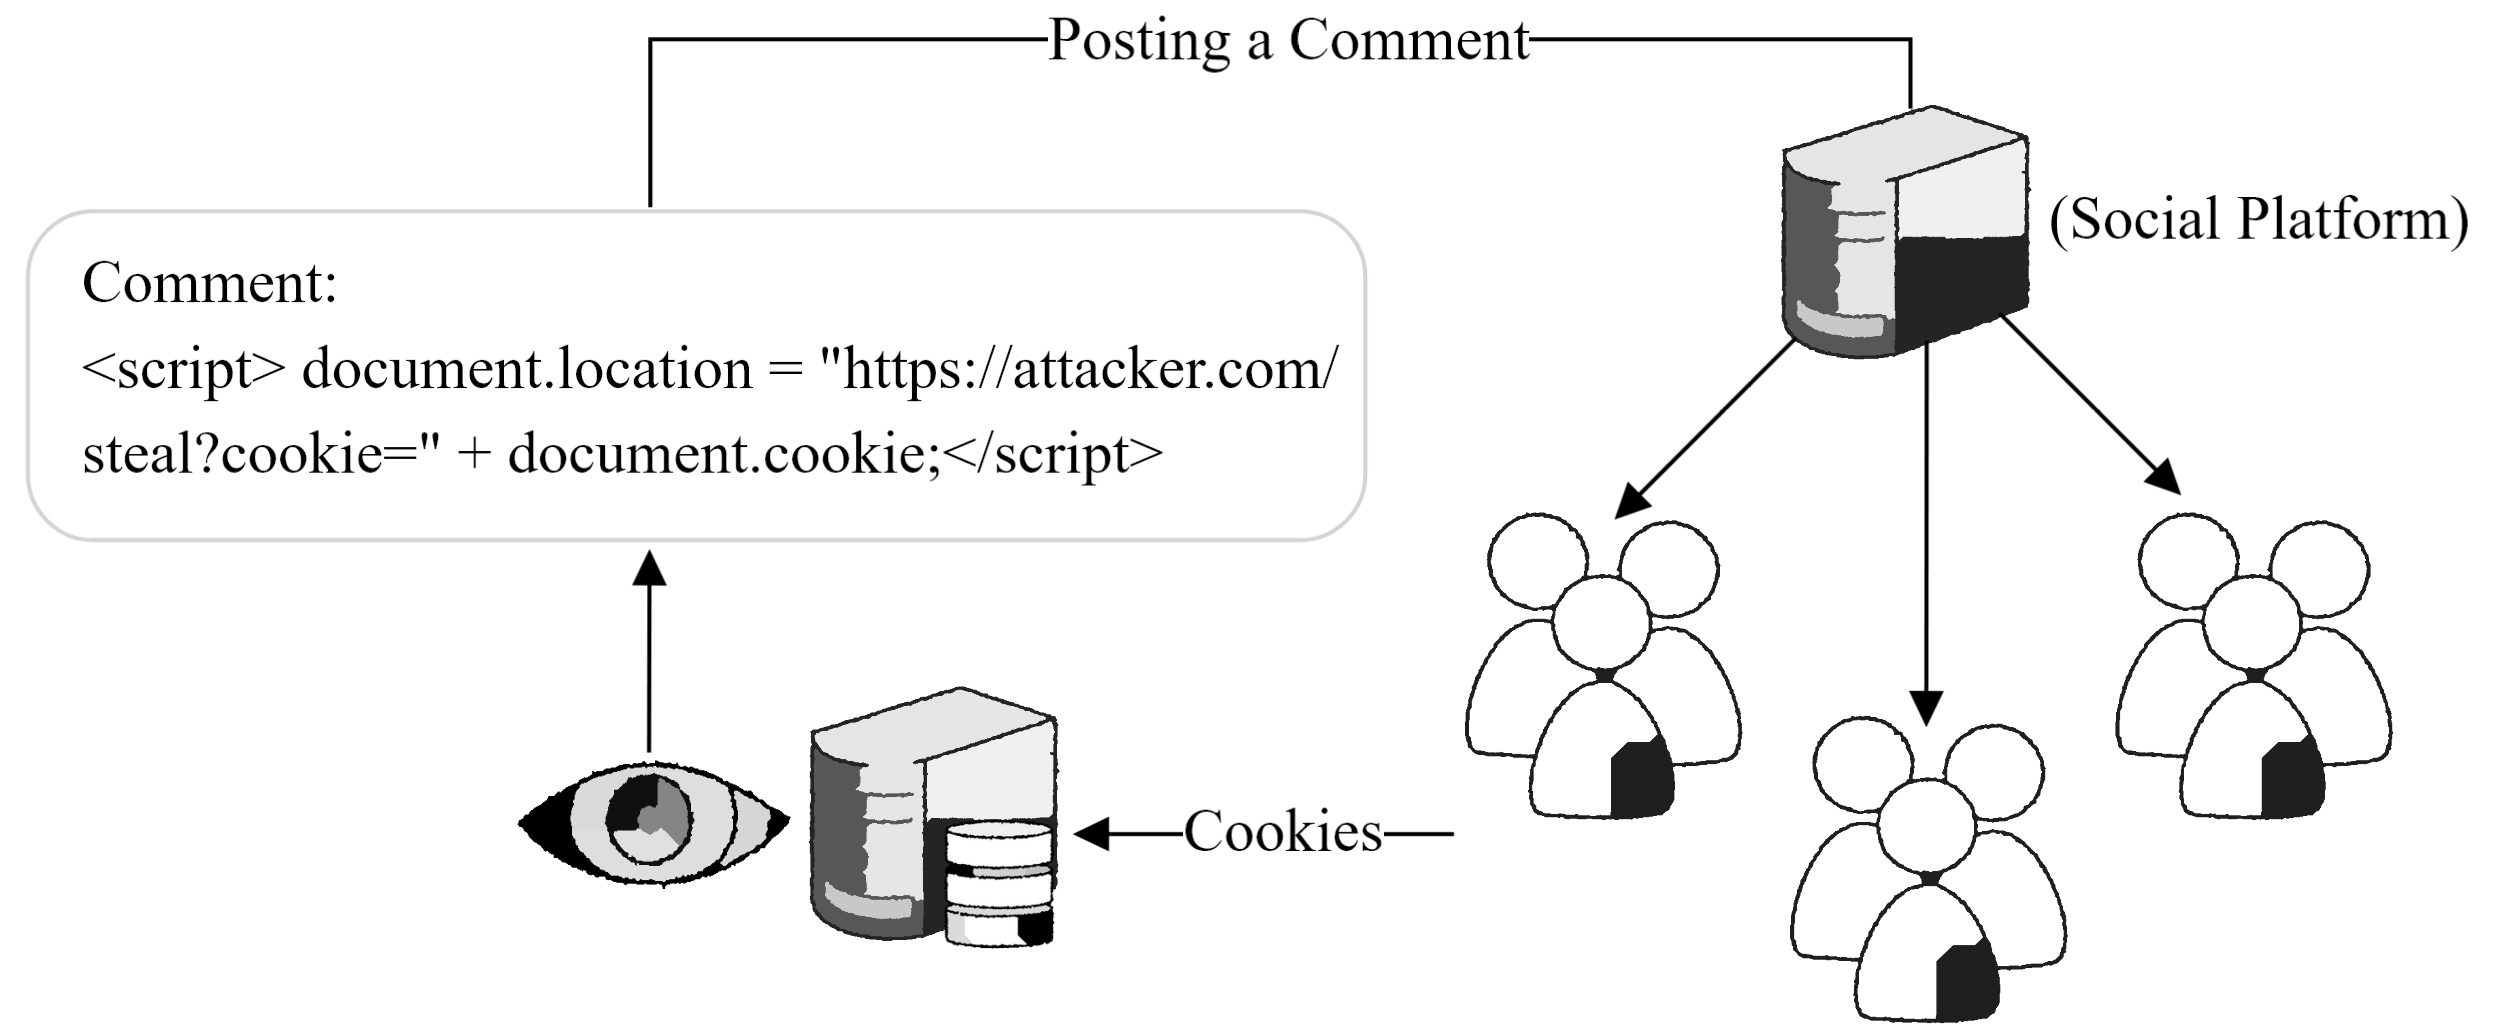
\includegraphics[width=.9\textwidth]{Sections/attk/cookie.png}
    \caption{A \textbf{Stored XSS} attack via posting a comment containing malicious code.}
    \label{fig:cookies}
\end{figure}

\newpage 

\noindent
The following attack uses both \textbf{Stored XSS} and \textbf{CSRF} to steal a user's session cookie:\\

\vspace{1em}


\begin{figure}[h!]
    \centering
    \hspace{-3em}
    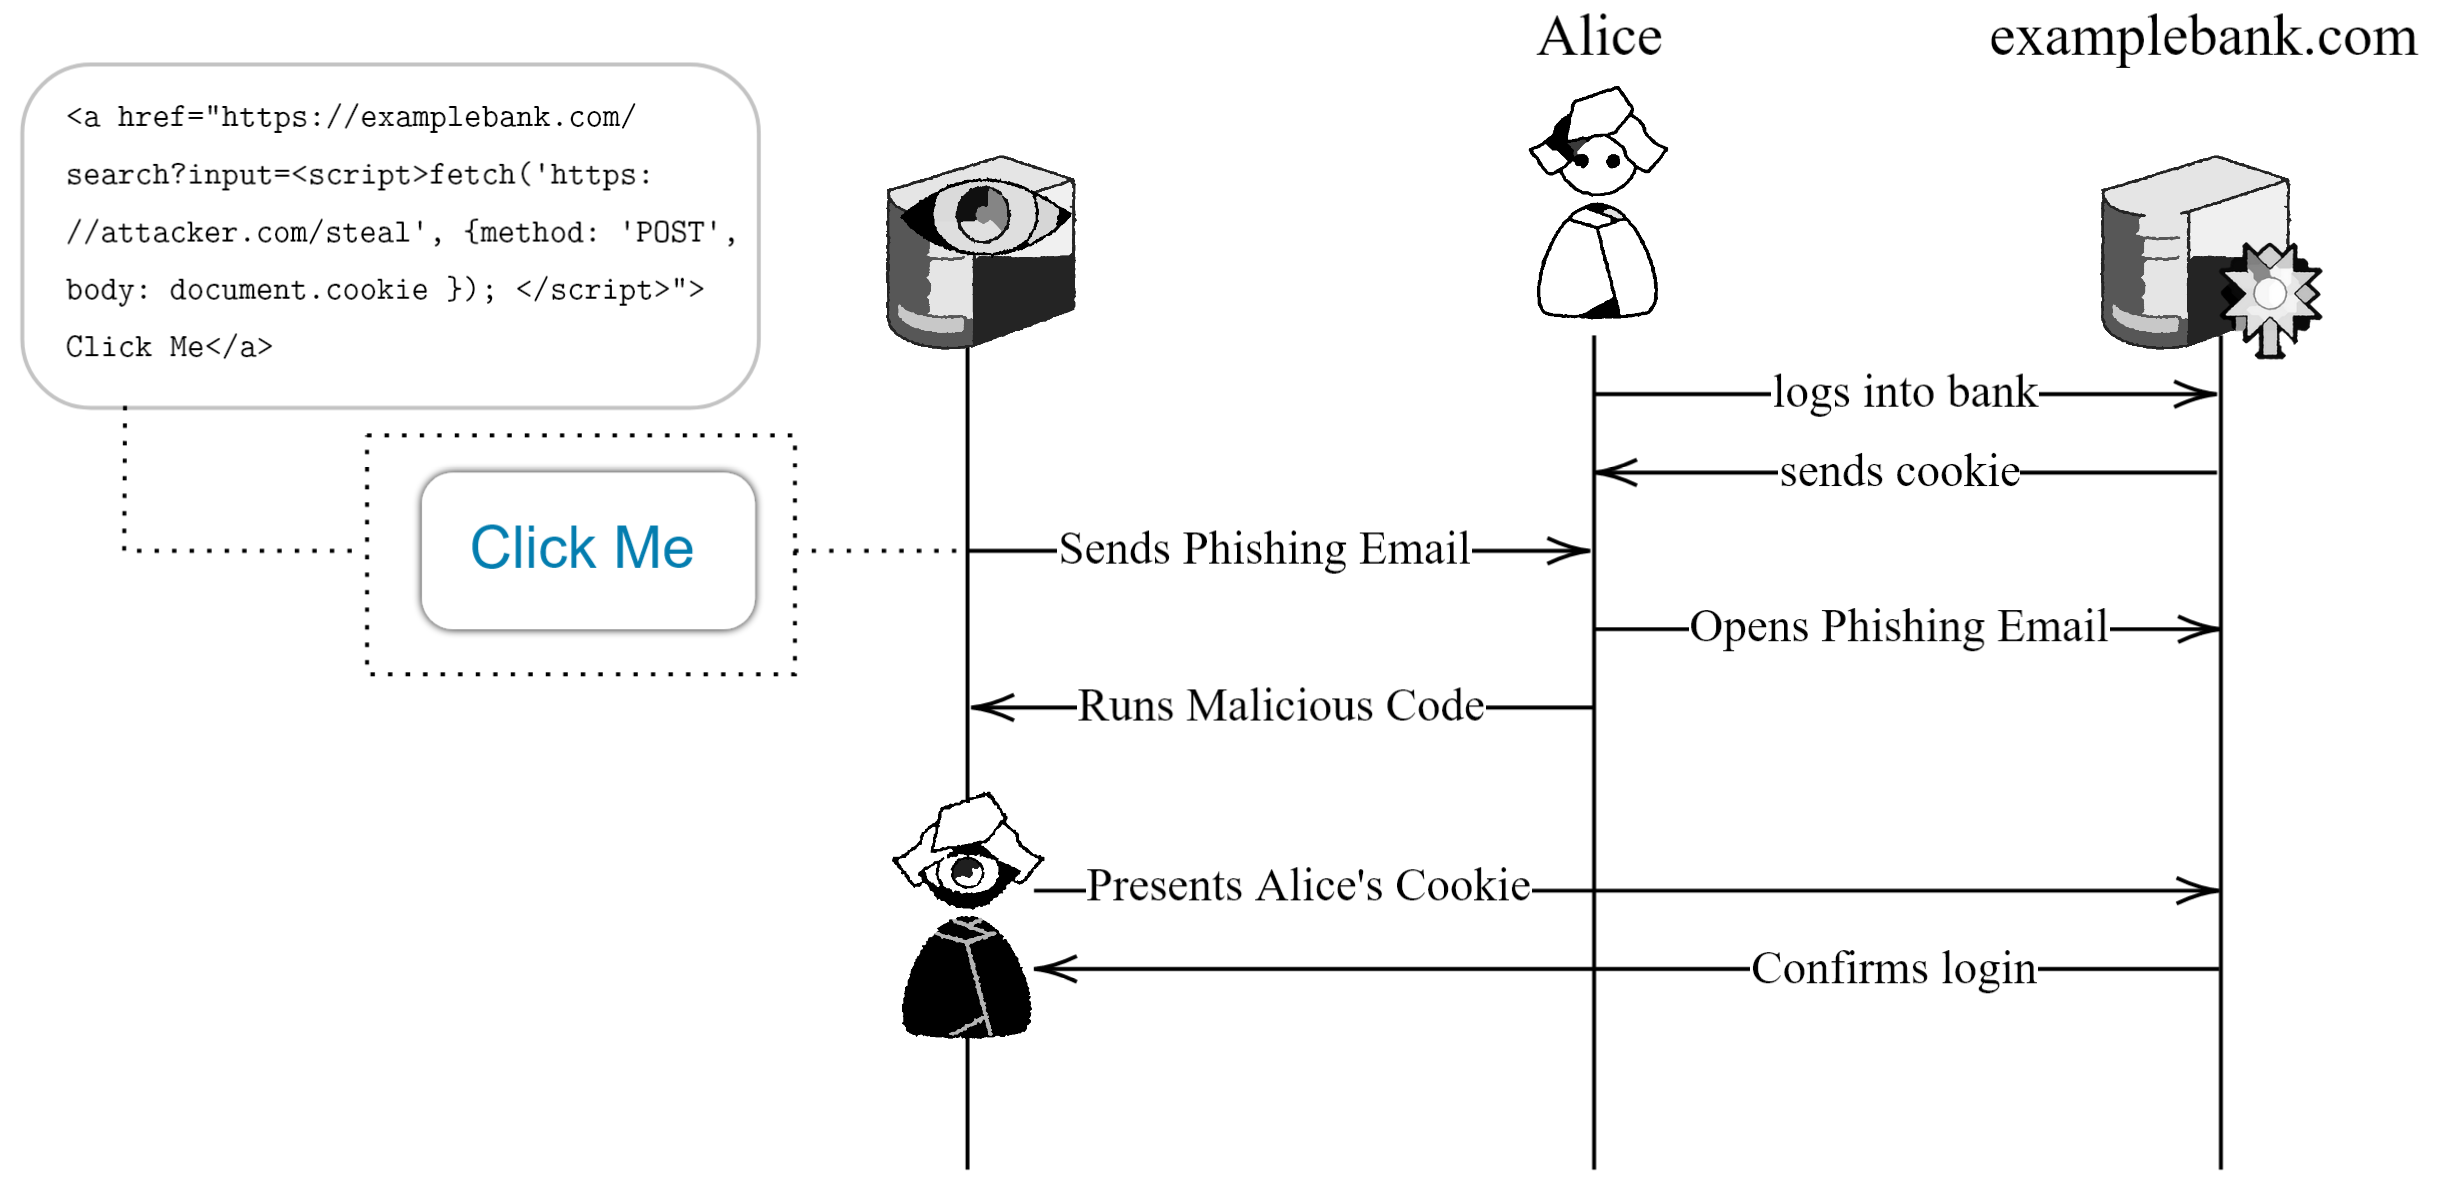
\includegraphics[width=1\textwidth]{Sections/attk/both.png}
    \caption{A \textbf{CSRF} attack via a malicious link.}
    \label{fig:csrf}
\end{figure}

\noindent
This attack can be easily thwarted by making cookies \textbf{HttpOnly}. Remember, \textbf{HttpSecure}
ensures that the cookie is only sent over HTTPS connections, nothing else.

\begin{theo}[Password Attacks]
    
    \label{theo:password_attacks}  
    Password attacks exploit weak, reused, or poorly managed passwords to gain unauthorized access. Common types include:  
    
    \begin{itemize}  
        \item \textbf{Credential Stuffing:} Using leaked username-password pairs from data breaches to access other accounts where users reused credentials.  
        \item \textbf{Dictionary Attacks:} Automated guessing of passwords using common words, phrases, or precomputed password lists.  
        \item \textbf{Fake Login Pages (Phishing):} Tricking users into entering passwords on fraudulent pages that mimic legitimate websites.  
        \item \textbf{Social Engineering:} Manipulating users into revealing passwords through deception, trust exploitation, or psychological tactics.  
    \end{itemize}  
    
    These attacks emphasize the importance of unique, strong passwords, user awareness, and multi-factor authentication (MFA) to mitigate risks.  
    
\end{theo}
    